\documentclass{beamer}
%\documentclass[handout]{beamer}

\usetheme[hidefootline,altlogo=images/ssl-logo_text.png,sidebarwidth=1.9cm]{Oxford}
\usepackage{subcaption}
\usepackage{listings}
\lstset{escapeinside={<@}{@>}}

\begin{document}

\bgroup
\let\oldfootnoterule\footnoterule
\setbeamerfont{footnote}{size=\tiny}

\title[Spoofing Earth Observation Satellites through Radio Overshadowing]{Firefly: Spoofing Earth Observation Satellites through Radio Overshadowing}
\author[Edd Salkield]{
  \emph{Edd Salkield}
  \inst{1}
  \and
  Joshua Smailes
  \inst{1}
  \and
  Sebastian Köhler
  \inst{1}
  \and
  Simon Birnbach
  \inst{1}
  \and
  Richard Baker
  \inst{1}
  \and
  Martin Strohmeier
  \inst{2}
  \and
  Ivan Martinovic
  \inst{1}
}
\institute[--~~Systems Security Lab]{
  \inst{1} Systems Security Lab, University of Oxford \and %
  \inst{2} Cyber-Defence Campus, armasuisse Science + Technology
}
\date{Trinity Term 2022}

\makeoxfordtitle

\note{
Satellite data is becoming increasingly important in private enterprises, research applications, and in coordinating national responses to events such as forest fires.
However, many of these satellites downlink this data on unauthenticated wireless channels.
This opens the door for spoofing attacks, where an adversary can impersonate a legitimate satellite by using a software-defined radio to transmit a malicious signal, which is received and decoded by the victim ground station as though it were legitimate.

Hi, my name's Edd Salkield, and I'm presenting to you today Firefly, a paper from the Systems Security Lab at the University of Oxford.
In this talk, we'll provide an overview of our research into the vulnerability of current Earth observation satellite systems to spoofing attacks, with more details found in the paper.
Taking NASA's live forest fire detection system as a case study, we demonstrate that the attacker can arbitrarily manipulate fires in the derived dataset to trigger false emergency response or mislead crisis analysis, and achieve denial of service in the processing software.
We conclude with a discussion of physical-layer countermeasures to detect and defend against spoofing, even when the satellite hardware cannot be upgraded.
}

\section{Motivation}
\subsection{Challenges}

\def\footnoterule{\only<6->\oldfootnoterule}
\begin{frame}
  \frametitle{Challenges of unauthenticated satellites}
  \begin{itemize}[<+->]
    \item Many current satellites do not encrypt the downlink, due to:
    \begin{itemize}[<+->]
      \item Increased power budget and costs
      \item Open access data
      \item Legacy systems backwards compatibility
    \end{itemize}
    
    \item Other satellites are decryptable, due to:
    \begin{itemize}[<+->]
      \item Insecure cryptosystems~\footnote<6->{COMS-1 uses single DES \url{https://vksdr.com/lrit-key-dec/}}
      \item Leaked keys~\footnote<7->{GK-2A keys leaked in source code \url{https://vksdr.com/xrit-rx/}}
    \end{itemize}
  \end{itemize}
\end{frame}

\begin{frame}
  \frametitle{Challenges of unauthenticated satellites}
  \framesubtitle{Insecure Earth Observation Satellites}

  Satellites with insecure downlinks include:

  \begin{itemize}
    \item \textbf{Fire detection and management}, e.g., Terra, Aqua
    \pause
    \item Geospatial intelligence, e.g., Landsat-7..9
    \item Weather monitoring, e.g., GOES-14..17, FengYun series
    \item Infrared sensing, e.g., Metop-A,B
    \item Climate monitoring, e.g., Suomi-NPP
  \end{itemize}

  \pause
  \newline
  Further details available in the paper
\end{frame}

\subsection{Implications}

\def\footnoterule{\only<3->\oldfootnoterule}
\begin{frame}
  \frametitle{Implications}
  \framesubtitle{Data secrecy}

  \begin{center}
    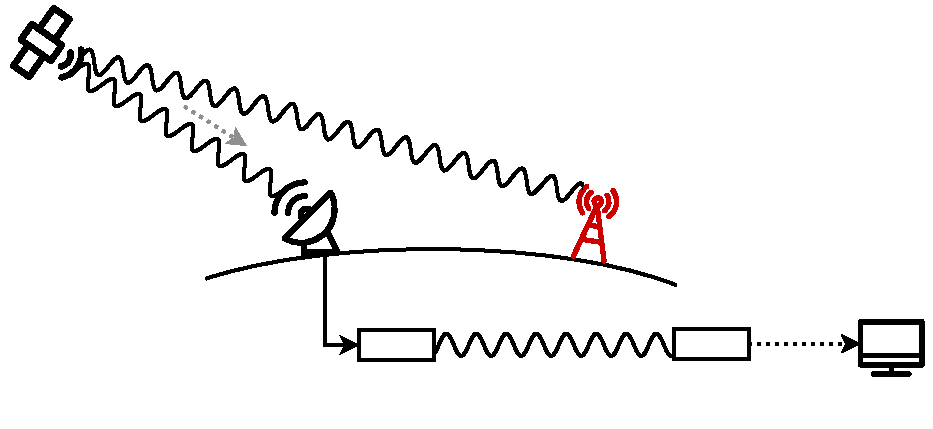
\includegraphics[width=0.7\textwidth]{images/eavesdropping_illustration.pdf}
  \end{center}

  \pause

  Using an SDR and open source software, attackers can:
  \pause
  \begin{itemize}[<+->]
    \item Read confidential maritime data\footnote<3->[1]{Pavur et al. (2020) ``\textit{A Tale of Sea and Sky on the Security of Maritime VSAT Communications}''} and internet traffic\footnote<3->[2]{Pavur et al. (2019) ``\textit{Secrets in the Sky: On Privacy and Infrastructure Security in DVB-S Satellite Broadband}''}
    \item Eavesdrop on Iridium traffic and calls~\footnote<4->[3]{muccc ``\textit{Iridium Toolkit}'' \url{https://github.com/muccc/iridium-toolkit}}
  \end{itemize}
\end{frame}

\def\footnoterule{\only<5->\oldfootnoterule}
\begin{frame}
  \frametitle{Implications}
  \framesubtitle{Data authenticity and integrity}

  \vspace{-0.4cm}
  \begin{center}
    \includegraphics<1|handout:0>[width=0.7\textwidth]{images/overshadow_illustration_1.pdf}%
    \includegraphics<2|handout:0>[width=0.7\textwidth]{images/overshadow_illustration_2.pdf}%
    \includegraphics<3->[width=0.7\textwidth]{images/overshadow_illustration_3.pdf}%
  \end{center}

  \pause[4]
  \vspace{-0.5cm}
  Spoofing attacks have been shown against:

  \pause
  \begin{itemize}[<+->]
    \item GNSS to manipulate calculated location\footnote<5->[1]{Motallebighomi et. al. (2022) ``\textit{Cryptography Is Not Enough: Relay Attacks on Authenticated GNSS Signals}''}
    \item Uplinks for satellite hijacking\footnote<6->[2]{``\textit{2011 REPORT TO CONGRESS of the U.S.-CHINA ECONOMIC AND SECURITY REVIEW COMMISSION}'' p.223--224} or broadcast intrusion\footnote<6->[3]{Broadcasting (1986) ``\textit{'Captain Midnight' unmasked}''}
  \end{itemize}

  \pause[\thebeamerpauses]
  No work considers spoofing Earth Observation satellites

  \pause
  \textbf{RQ}: What can the attacker achieve by exploiting the unauthenticated channel?
\end{frame}

\subsection{Threat model}
\begin{frame}
  \frametitle{Threat model}

  \begin{center}
    \includegraphics<1|handout:0>[width=0.7\textwidth]{images/attack_illustration_1.pdf}%
    \includegraphics<2|handout:0>[width=0.7\textwidth]{images/attack_illustration_2.pdf}%
    \includegraphics<3->[width=0.7\textwidth]{images/attack_illustration_3.pdf}%
  \end{center}

  Attacker transmits counterfeit signals in the vicinity of the receiver, to:
  \begin{itemize}
    \item<2-> Affect the satellite-derived datasets
    \item<3> Exploit or disrupt downlink processing stages
  \end{itemize}
\end{frame}

\subsection{Attacker capabilities}

\def\footnoterule{\oldfootnoterule}
\begin{frame}
  \frametitle{Attacker capabilities}
  \framesubtitle{Estimated cost}

  \begin{center}
  \begin{tabular}{ l | l }
    \textbf{Hardware component} & \textbf{Cost} \\
    \hline
    \textit<2>{limeSDR} & $598$ USD \\
    \textit<3>{X-Band upconverter} & $100$ USD\footnotemark[1] \\
    \textit<4>{X-Band amplifier} & $1,638$ USD \\
    \textit<5>{Compatible antenna} & $431$ USD \\
    \hline
    \textit<6>{Total} & $3,000$ USD
  \end{tabular}
  \end{center}

  \footnotetext[1]{Estimated price from self-built amateur radio equipment}

  \pause[6]
  Within the budget of a motivated hobbyist
\end{frame}

\section{Case Study: FIRMS}
\subsection{Experiment setup}

\begin{frame}
  \frametitle{Case Study: Forest fire detection in FIRMS}
  \framesubtitle{NASA's global fire detection service}
  \centering
  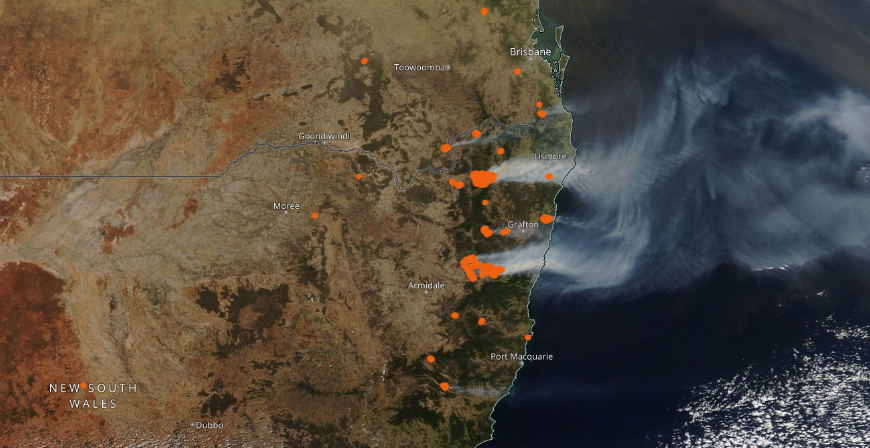
\includegraphics[width=\columnwidth]{images/bushfire.png}
  \newline
  The 2019 Australia bushfires as seen from Aqua's MODIS instrument, annotated with the \textit{Fires and Thermal Anomalies} dataset on NASA's worldview.
\end{frame}

\begin{frame}
  \frametitle{Case Study: Forest fire detection in FIRMS}
  \framesubtitle{Experiment setup}

  \begin{center}
    \includegraphics<1|handout:0>[width=0.8\textwidth]{images/attack_types_1.pdf}%
    \includegraphics<2|handout:0>[width=0.8\textwidth]{images/attack_types_2.pdf}%
    \includegraphics<3|handout:0>[width=0.8\textwidth]{images/attack_types_3.pdf}%
    \includegraphics<4->[width=0.8\textwidth]{images/attack_types_4.pdf}%
  \end{center}
  With a research account, anyone can download the entire set of decoding software from NASA's \textit{Direct Readout Laboratory}
  \url{https://directreadout.sci.gsfc.nasa.gov/}
\end{frame}

\subsection{Attack overview}

\def\footnoterule{\oldfootnoterule}
\begin{frame}
  \frametitle{Attack overview}
  \begin{itemize}[<+->]
    \item Obtain legitimate data from digital archive\footnote<1->[1]{\url{https://ladsweb.modaps.eosdis.nasa.gov/archive/}}
   \item Perform security audit on downlink decoder software\footnote<2->[2]{\url{https://directreadout.sci.gsfc.nasa.gov/}, with an academic account}
   \begin{itemize}
     \item Determine data integrity checks
     \item Identify vulnerabilities where safe input data assumed
   \end{itemize}
    \item Process data to add/remove artifacts\footnote<5->[3]{Code provided in the paper}
    \begin{itemize}
      \item Edit image format to insert fictitious data
      \item Construct payload packet to trigger vulnerability chain
    \end{itemize}
  \end{itemize}
\end{frame}


\subsection{Affecting the derived dataset}

\begin{frame}
  \frametitle{Affecting the derived dataset}
  \framesubtitle{Packet structure}
  \includegraphics<1|handout:0>[width=\textwidth]{images/packet_image_1.pdf}%
  \includegraphics<2|handout:0>[width=\textwidth]{images/packet_image_2.pdf}%
  \includegraphics<3|handout:0>[width=\textwidth]{images/packet_image_3.pdf}%
  \includegraphics<4>[width=\textwidth]{images/packet_image_4.pdf}%
\end{frame}

\begin{frame}
  \frametitle{Affecting the derived dataset}
  \framesubtitle{Attack consequences}
  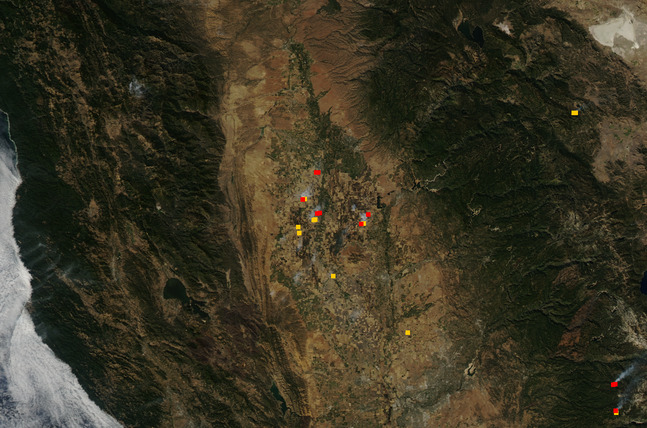
\includegraphics[width=\textwidth]{images/injection/original.jpg}
  \newline
  \centering
  Original image.
\end{frame}

\begin{frame}
  \frametitle{Affecting the derived dataset}
  \framesubtitle{Attack consequences}
  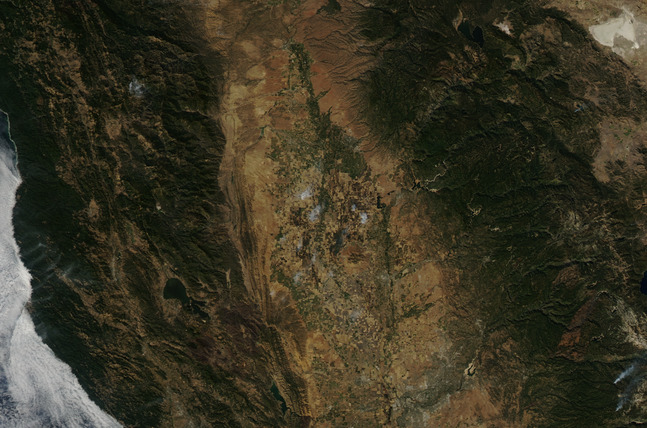
\includegraphics[width=\textwidth]{images/injection/masked_0.jpg}
  \newline
  \centering
  Masking existing fires.
\end{frame}

\begin{frame}
  \frametitle{Affecting the derived dataset}
  \framesubtitle{Attack consequences}
  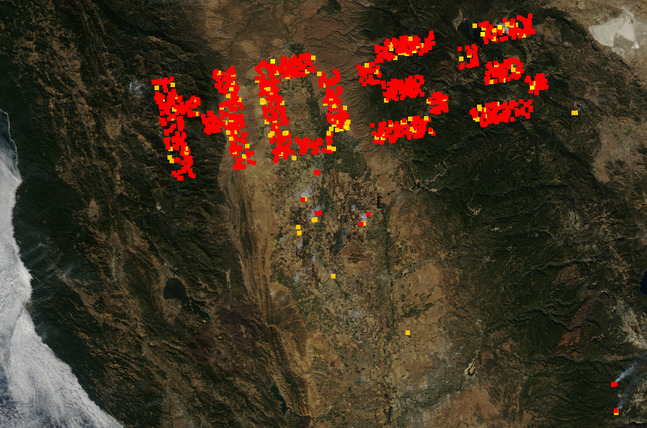
\includegraphics[width=\textwidth]{images/injection/pixels_800_140.jpg}
  \newline
  \centering
  Fine-grained control over fire injection.
\end{frame}

\subsection{Exploiting the decoder}

\begin{frame}
  \frametitle{Exploiting the decoder}
  \framesubtitle{Packet structure}
  \includegraphics<1|handout:0>[width=\textwidth]{images/packet_data_1.pdf}%
  \includegraphics<2|handout:0>[width=\textwidth]{images/packet_data_2.pdf}%
  \includegraphics<3->[width=\textwidth]{images/packet_data_3.pdf}%
\end{frame}

\begin{frame}[fragile]
  \frametitle{Exploiting the decoder}
  \framesubtitle{Attack consequences}
  \begin{lstlisting}[basicstyle=\ttfamily\small,basewidth=0.6em]
$ printf %1337s  | tr " " "f"  | \
  spppack --type-flag telecommand \
            --sec-hdr-flag 1 \
            --app-id aqua_modis \
  > bad_packet.PDS
  \end{lstlisting}

  \pause
  \begin{lstlisting}[basicstyle=\ttfamily\small,basewidth=0.6em]
$ cat bad_packet.PDS good_packet_sequence.PDS \
    > ./data/MYD00F.A2015299...001.PDS
  \end{lstlisting}

  \pause
  \begin{lstlisting}[basicstyle=\ttfamily\small,basewidth=0.6em]
$ ./run_all.sh ./data/
DATA_PATH: /mnt/data
CONTAINER_RUNTIME: docker
  \end{lstlisting}

  \pause
  \begin{lstlisting}[basicstyle=\ttfamily\small,basewidth=0.6em]
### Processing new PDS:
  MYD00F.A2015299.2110.20152992235.001.PDS
  \end{lstlisting}

  \pause
  \begin{lstlisting}[basicstyle=\ttfamily\small,basewidth=0.6em]
### Running modisl1db l1a-geo initial processing
<@\textcolor{red}{l0fix\_modis: Unrecoverable error in l0fix\_modis!}@>
  \end{lstlisting}
\end{frame}

\section{Countermeasures}

\def\footnoterule{\only<5->\oldfootnoterule}
\begin{frame}
  \frametitle{Countermeasures}

  Cryptography should be required in future satellites

  \pause
  But existing satellites can't be upgraded
  \newline

  \pause
  Backwards-compatible countermeasures:

  \pause
  \begin{itemize}[<+->]
    \item{Multi-receiver data comparison}
    \item{Timing analysis}\footnote<5->[2]{Jedermann et. al. (2021) ``\textit{Orbit-based Authentication Using TDOA Signatures in Satellite Networks}''}
    \item{Physical-layer fingerprinting}\footnote<6->[3]{Oligeri et. al. (2022) ``\textit{PAST-AI: Physical-Layer Authentication of Satellite Transmitters via Deep Learning}''}
  \end{itemize}
  \newline

  \pause[\thebeamerpauses]
  Comparative analysis presented in the paper

  \note{
    Multi-receiver data comparison
    \begin{itemize}
      \item Certain systems already have multiple receiver stations
      \item Protects against decoder exploitation
      \item Doesn't require any hardware modifications to the receiver
    \end{itemize}

    Timing analysis
    \begin{itemize}
      \item Triangulating the source effective in other systems such as aircraft
      \item Calculated position can be compared against orbital parameters
      \item Requires accurate clock synchronisation and multiple receivers
    \end{itemize}

    Physical-layer fingerprinting
    \begin{itemize}
      \item Analyse properties of the legitimate/overshadowed signal
      \item Only effective on the downlink
      \item Traditional approaches like analysing signal-to-noise may prove effective
      \item New ML approaches starting to be created (PAST-AI)
    \end{itemize}
  }
\end{frame}

\section{Conclusion}

\begin{frame}
  \frametitle{Conclusion}

  Our paper...
  \pause
  \begin{itemize}[<+->]
    \item presents a demonstration of byte-level spoofing against NASA's forest fire detection system.
    \item provides the source code required to manipulate the packet data and structure.
    \item confirms that only a moderate budget is required to perform these attacks.
    \item identifies current countermeasures which significantly increase attack difficulty.
  \end{itemize}
\end{frame}

\begin{frame}
  \frametitle{Thank you for your attention}

  \vspace{-1.2cm}
  \begin{center}
    \Large
    Any questions?
  \end{center}
  \vspace{1cm}

  \begin{center}
    Reach out to me at \\
    \textit{edd.salkield@cs.ox.ac.uk}
  \end{center}
\end{frame}
\end{document}
